\documentclass[12pt,a4paper]{article}
\usepackage{fontspec}
\setmainfont{Noto Serif}
\setsansfont{Noto Sans}
\usepackage[english,russian]{babel}
\usepackage[a4paper,left=25mm,right=15mm,top=20mm,bottom=20mm]{geometry}
\usepackage{amsmath,amssymb,booktabs,longtable,tabularx,array,graphicx,float,caption,enumitem,hyperref,fancyhdr,indentfirst}
\usepackage{setspace}
\onehalfspacing
\setlength{\parindent}{1.25cm}
\setlength{\parskip}{0pt}
\graphicspath{{./}}
\hypersetup{hidelinks}
\captionsetup{font=small,labelsep=endash,justification=centering}
\addto\captionsrussian{\renewcommand{\figurename}{Рисунок}\renewcommand{\tablename}{Таблица}}
\renewcommand{\tablename}{Таблица}
\pagestyle{fancy}\fancyhf{}\fancyfoot[C]{\thepage}\renewcommand{\headrulewidth}{0pt}
\setcounter{tocdepth}{2}
\begin{document}
\begin{titlepage}
\begin{center}
{\small САНКТ-ПЕТЕРБУРГСКИЙ ГОСУДАРСТВЕННЫЙ УНИВЕРСИТЕТ\\ Математико-механический факультет}
\vfill
{\bfseries\Large ОТЧЁТ}\\[1em]
по задаче курса «Машинное обучение»\\[1.5em]
{\bfseries\large ПРОГНОЗ ОСТАТОЧНОГО РЕСУРСА\\ АВИАЦИОННОГО ДВИГАТЕЛЯ}\\[0.8em]
(вариант 12, набор данных NASA C-MAPSS FD001)\\[1em]
Регрессия, обучение MLP и исследование гиперпараметров
\end{center}
\vfill
\begin{flushright}
Выполнил: студент группы 23.Б12\\ Бирклин Артур (st117157)
\end{flushright}
\vfill
\begin{center}Санкт-Петербург\\2026\end{center}
\end{titlepage}
\setcounter{page}{2}
\section*{РЕФЕРАТ}\addcontentsline{toc}{section}{Реферат}
Исследуется прогноз остаточного ресурса (Remaining Useful Life, RUL) авиационного двигателя по рабочим условиям и датчикам в симуляторе NASA C-MAPSS FD001. Цель работы — установить, позволяет ли многослойный персептрон (MLP) извлекать информацию о деградации сверх простой модели возраста двигателя, и оценить поведение моделей при малом RUL. Сравниваются возрастная регрессия, Ridge и две конфигурации MLP. В дополнение к первоначальному эксперименту рассматриваются обучение MLP, сетка из восьми конфигураций архитектуры, регуляризации и скорости обучения, три независимых разбиения по двигателям, пять вариантов ограничения обучающего RUL (100, 125, 150, 200 и без ограничения), процентные метрики и насыщение качества.

Для основного эксперимента использованы 40 полных обучающих траекторий (7\,954 цикла), 20 других двигателей для валидации (4\,070 циклов), а также 100 отдельных тестовых двигателей с известными RUL только для последних доступных строк. Исходная MLP с датчиками и номером цикла достигла MAE = 19,46 цикла на штатном тесте против 29,15 цикла у возрастной модели; при RUL не более 30 ошибка уменьшилась с 32,57 до 9,24 цикла. Дополнительное исследование выявило зависимость результата от состава двигателей и неоднозначный эффект ограничения RUL сверху: точность у близких к отказу двигателей иногда возрастает, но полная MAE на неограниченной шкале может ухудшиться.

\textbf{Ключевые слова:} NASA C-MAPSS, FD001, RUL, многослойный персептрон, регрессия, подбор гиперпараметров, MAE, RMSE, MAPE, деградация двигателя.
\newpage
\tableofcontents
\newpage
\section*{ВВЕДЕНИЕ}\addcontentsline{toc}{section}{Введение}
Задача прогнозирования остаточного ресурса возникает в предиктивном обслуживании технических систем: чем точнее оценено время до отказа, тем лучше можно планировать диагностику и замену узлов. При этом счётчик наработки сам по себе не описывает фактическое состояние двигателя, потому что интенсивность деградации зависит от индивидуальной траектории. Показания датчиков потенциально позволяют оценивать не только возраст, но и текущее состояние механизма.

Для проверки этого предположения выбран набор FD001 из NASA C-MAPSS. В отличие от данных реальной эксплуатации, это численно сгенерированные траектории, что накладывает ограничения на перенос выводов. Исследовательский вопрос формулируется так: \emph{насколько датчики улучшают прогноз по сравнению с одним циклом, особенно непосредственно перед отказом?}

В соответствии с вариантом 12 обучение ограничено максимум 8\,000 циклами, а разбиение на обучение и проверку проводится только по целым двигателям, без случайного распределения строк одного двигателя между наборами. Прогнозируется исходный остаточный ресурс; длина будущей траектории не вводится в признаки. Два обязательных графика демонстрируют прогнозы на полностью отложенных двигателях и ошибки по диапазонам истинного RUL.

После замечаний преподавателя также изучены кривые обучения MLP, настройка гиперпараметров, устойчивость по разным случайным разбиениям и влияние верхней границы RUL; добавлены процентные метрики. Везде различаются основной фиксированный тест и дополнительные валидационные эксперименты.
\section{Данные и протокол эксперимента}
\subsection{Структура FD001}
В архиве используются файлы \texttt{train\_FD001.txt}, \texttt{test\_FD001.txt}, \texttt{RUL\_FD001.txt}. Обучающая часть содержит 100 полных траекторий, всего 20\,631 запись. Тестовая часть содержит 100 обрывающихся траекторий. Каждая запись включает идентификатор двигателя, номер цикла, три параметра рабочих условий и 21 показатель датчиков. В FD001 моделируются один рабочий режим и один тип деградации (узел компрессора высокого давления).

Пусть $c_{ij}$ — наблюдаемый цикл $j$ двигателя $i$, $C_i$ — его последний цикл в полной обучающей траектории. Тогда целевое значение вычисляется как
\begin{equation}y_{ij}=\mathrm{RUL}_{ij}=C_i-c_{ij}.\end{equation}
Это определение применяется только для полных обучающих траекторий. На штатном тесте файл \texttt{RUL\_FD001.txt} задаёт эталон RUL исключительно для последней строки каждого двигателя. Включение $C_i$ или любых производных от будущей длительности в признаки не допускается.
\subsection{Разбиение и защита от утечки}
При исходном \texttt{seed=42} из 100 обучающих идентификаторов 20 целиком отведены на валидацию; из оставшихся выбраны 40 полных траекторий общей длиной 7\,954 цикла. Валидация включает 4\,070 циклов. Разбиение строго по \texttt{engine\_id}. Отдельные 100 тестовых двигателей используются только для финальной оценки уже заданных моделей.

Медианная импутация и стандартизация обучаются исключительно на обучающем подмножестве. Константные признаки выявляются также только на нём. Номер двигателя исключён из входных признаков. Номер цикла используется в отдельной конфигурации MLP и в возрастном базовом алгоритме.
\begin{table}[H]\centering\caption{Размеры частей данных в основном эксперименте}\begin{tabular}{lrrl}\toprule Часть & Двигатели & Циклы / строки & Назначение\\\midrule Обучение & 40 & 7\,954 & Настройка весов\\ Валидация & 20 & 4\,070 & Оценка и подбор\\ Штатный тест & 100 & 100 & Последний цикл каждого\\\bottomrule\end{tabular}\end{table}
\subsection{Целевая переменная с ограничением и без него}
В дополнительных экспериментах сравниваются исходная $y$ и ограниченная $y^{(c)}=\min(y,c)$ для $c\in\{100,125,150,200\}$. В обоих случаях качество рассчитывается по \emph{исходному, неограниченному} RUL валидационной части. Это принципиально важно: ограничение цели — гипотеза о режиме обучения, а не новая метрика и не подмена эталонного ответа. Оно может облегчать оценку близкого отказа, но ухудшать предсказания для молодых двигателей.
\section{Метрики и базовые алгоритмы}
Для фактических значений $y_i$ и прогнозов $\hat y_i$ использованы
\begin{align}
\mathrm{MAE}&=\frac1n\sum_{i=1}^n|y_i-\hat y_i|,\\
\mathrm{RMSE}&=\sqrt{\frac1n\sum_{i=1}^n(y_i-\hat y_i)^2},\\
\mathrm{MAPE}&=\frac{100\%}{|I_+|}\sum_{i\in I_+}\frac{|y_i-\hat y_i|}{y_i},\quad I_+=\{i:y_i>0\},\\
\mathrm{sMAPE}&=\frac{100\%}{n}\sum_{i=1}^n\frac{2|y_i-\hat y_i|}{|y_i|+|\hat y_i|}.
\end{align}
Для sMAPE нулевой знаменатель трактуется как нулевой вклад. Поскольку в полных траекториях присутствует $y_i=0$, MAPE по ним определяется только на наблюдениях $y_i>0$. Дополнительно приводится \emph{MAPE по $y_i\geq10$}, снижающая влияние очень малых знаменателей. Эти две версии не следует смешивать. Для официального теста среди последних точек нет истинного RUL, равного нулю.

Базовая возрастная модель — RandomForestRegressor из 100 деревьев с \texttt{min\_samples\_leaf=25}, вход — только номер цикла. Линейный базовый алгоритм — Ridge ($\alpha=100$) на рабочих условиях и датчиках. Нейросети сопоставляются с ними по одним и тем же строкам.
\section{Первоначальное сравнение моделей}
\begin{table}[H]\centering\caption{Качество на штатном тесте FD001, 100 двигателей}\begin{tabular}{lrr}\toprule Модель & MAE, циклы & RMSE, циклы\\\midrule Только цикл (случайный лес) & 29,15 & 35,14\\ Ridge, датчики и условия & 23,30 & 29,13\\ MLP, датчики и условия & 22,50 & 30,50\\ \textbf{MLP, датчики, условия и цикл} & \textbf{19,46} & \textbf{25,60}\\\bottomrule\end{tabular}\end{table}
Сенсорная MLP без возраста даёт уменьшение MAE на 22,8\% относительно возрастного алгоритма. Добавление номера цикла к тем же сенсорным признакам снижает MAE ещё на 13,5\% относительно сенсорной MLP. Общий выигрыш лучшей исходной модели против возрастной составляет около 33,3\%. Это сравнение получено при одном фиксированном разбиении; вывод об устойчивости требует дополнительных запусков.
\begin{figure}[p]\centering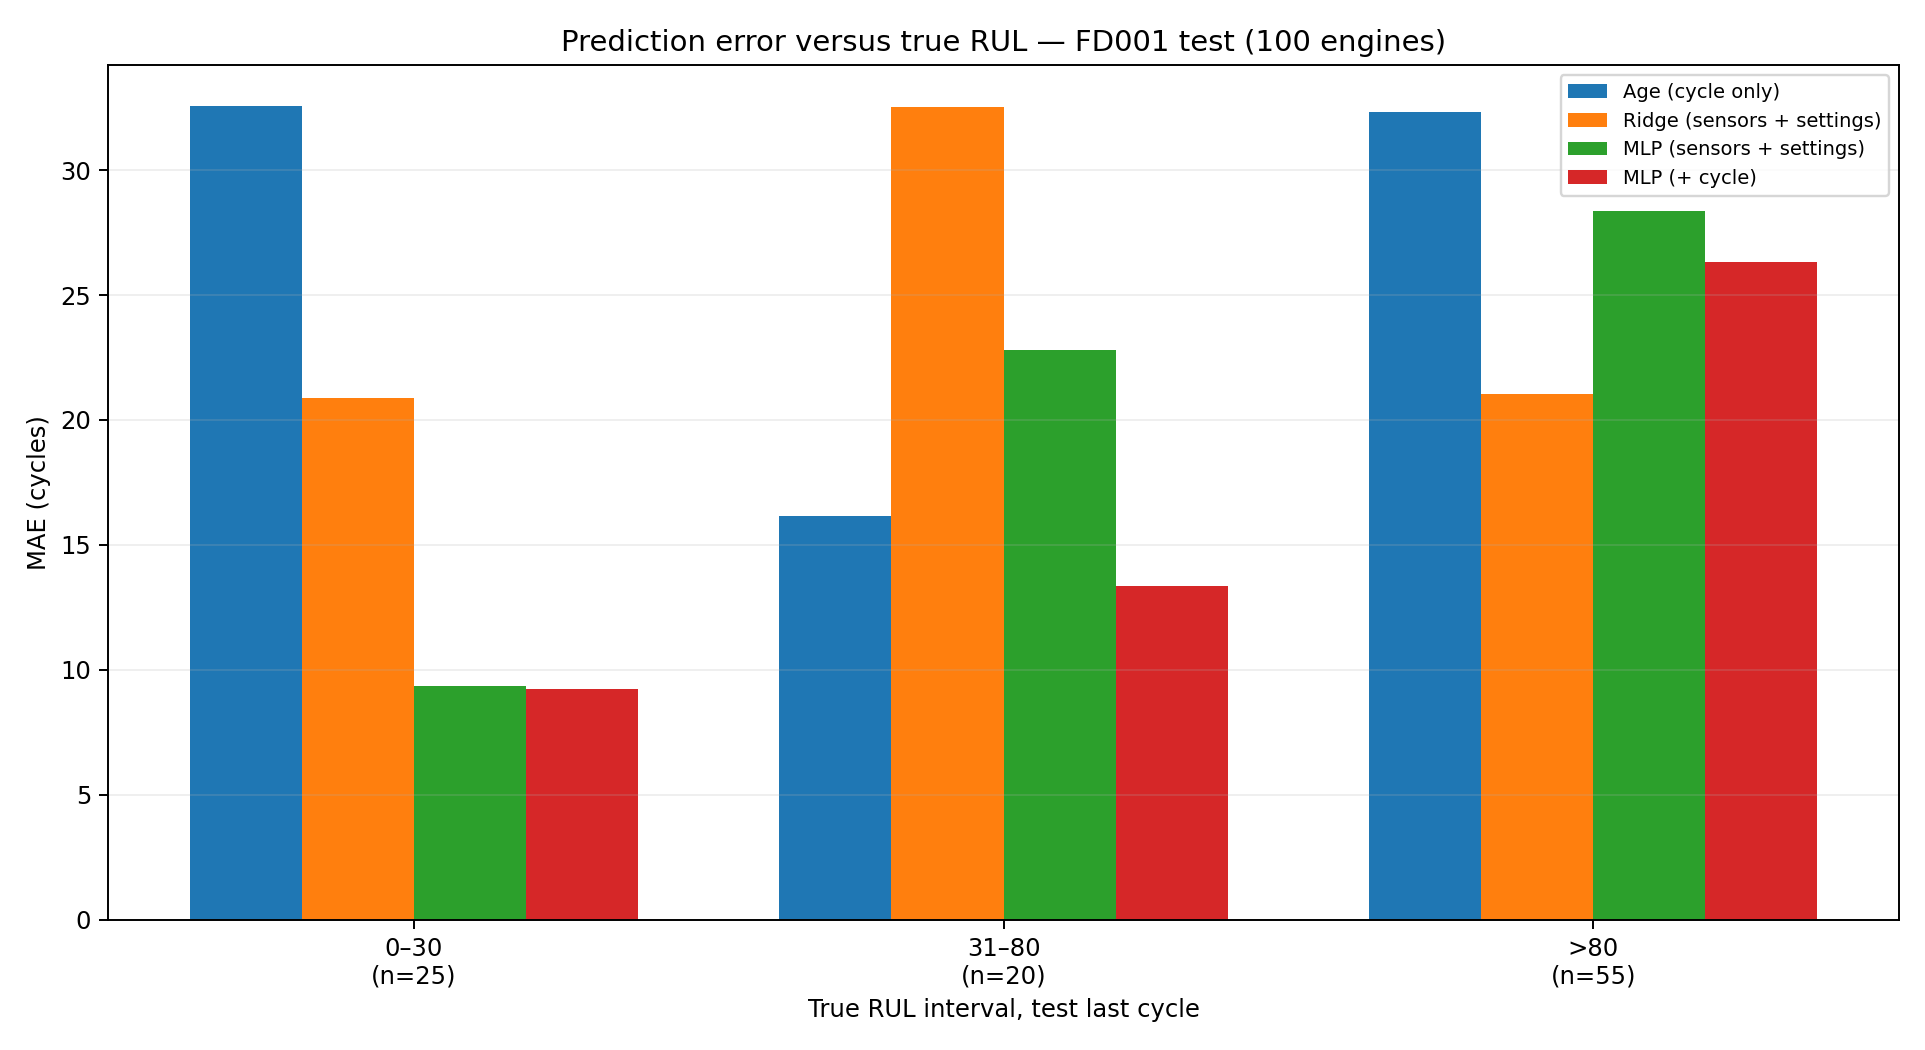
\includegraphics[width=.96\textwidth]{mae_by_rul.png}\caption{MAE на официальном тесте по диапазонам истинного RUL: 0--30 (25 двигателей), 31--80 (20), более 80 (55)}\end{figure}
\begin{table}[H]\centering\caption{MAE по диапазонам истинного RUL на официальном тесте}\begin{tabular}{lrrr}\toprule Модель & 0--30 & 31--80 & $>80$\\\midrule Только цикл & 32,57 & 16,15 & 32,33\\ Ridge & 20,88 & 32,51 & 21,05\\ MLP, датчики & 9,35 & 22,81 & 28,36\\ MLP, датчики и цикл & \textbf{9,24} & \textbf{13,36} & 26,32\\\bottomrule\end{tabular}\end{table}
При RUL не более 30 циклов сенсорная MLP улучшает MAE относительно возрастной модели примерно на 71,3\%, комбинированная — на 71,6\%. На больших значениях RUL преимущество становится менее однозначным: например, для диапазона 31--80 Ridge оказывается хуже возрастной модели. Это требует анализировать качество по состояниям двигателя, а не только по одной итоговой метрике.
\begin{figure}[p]\centering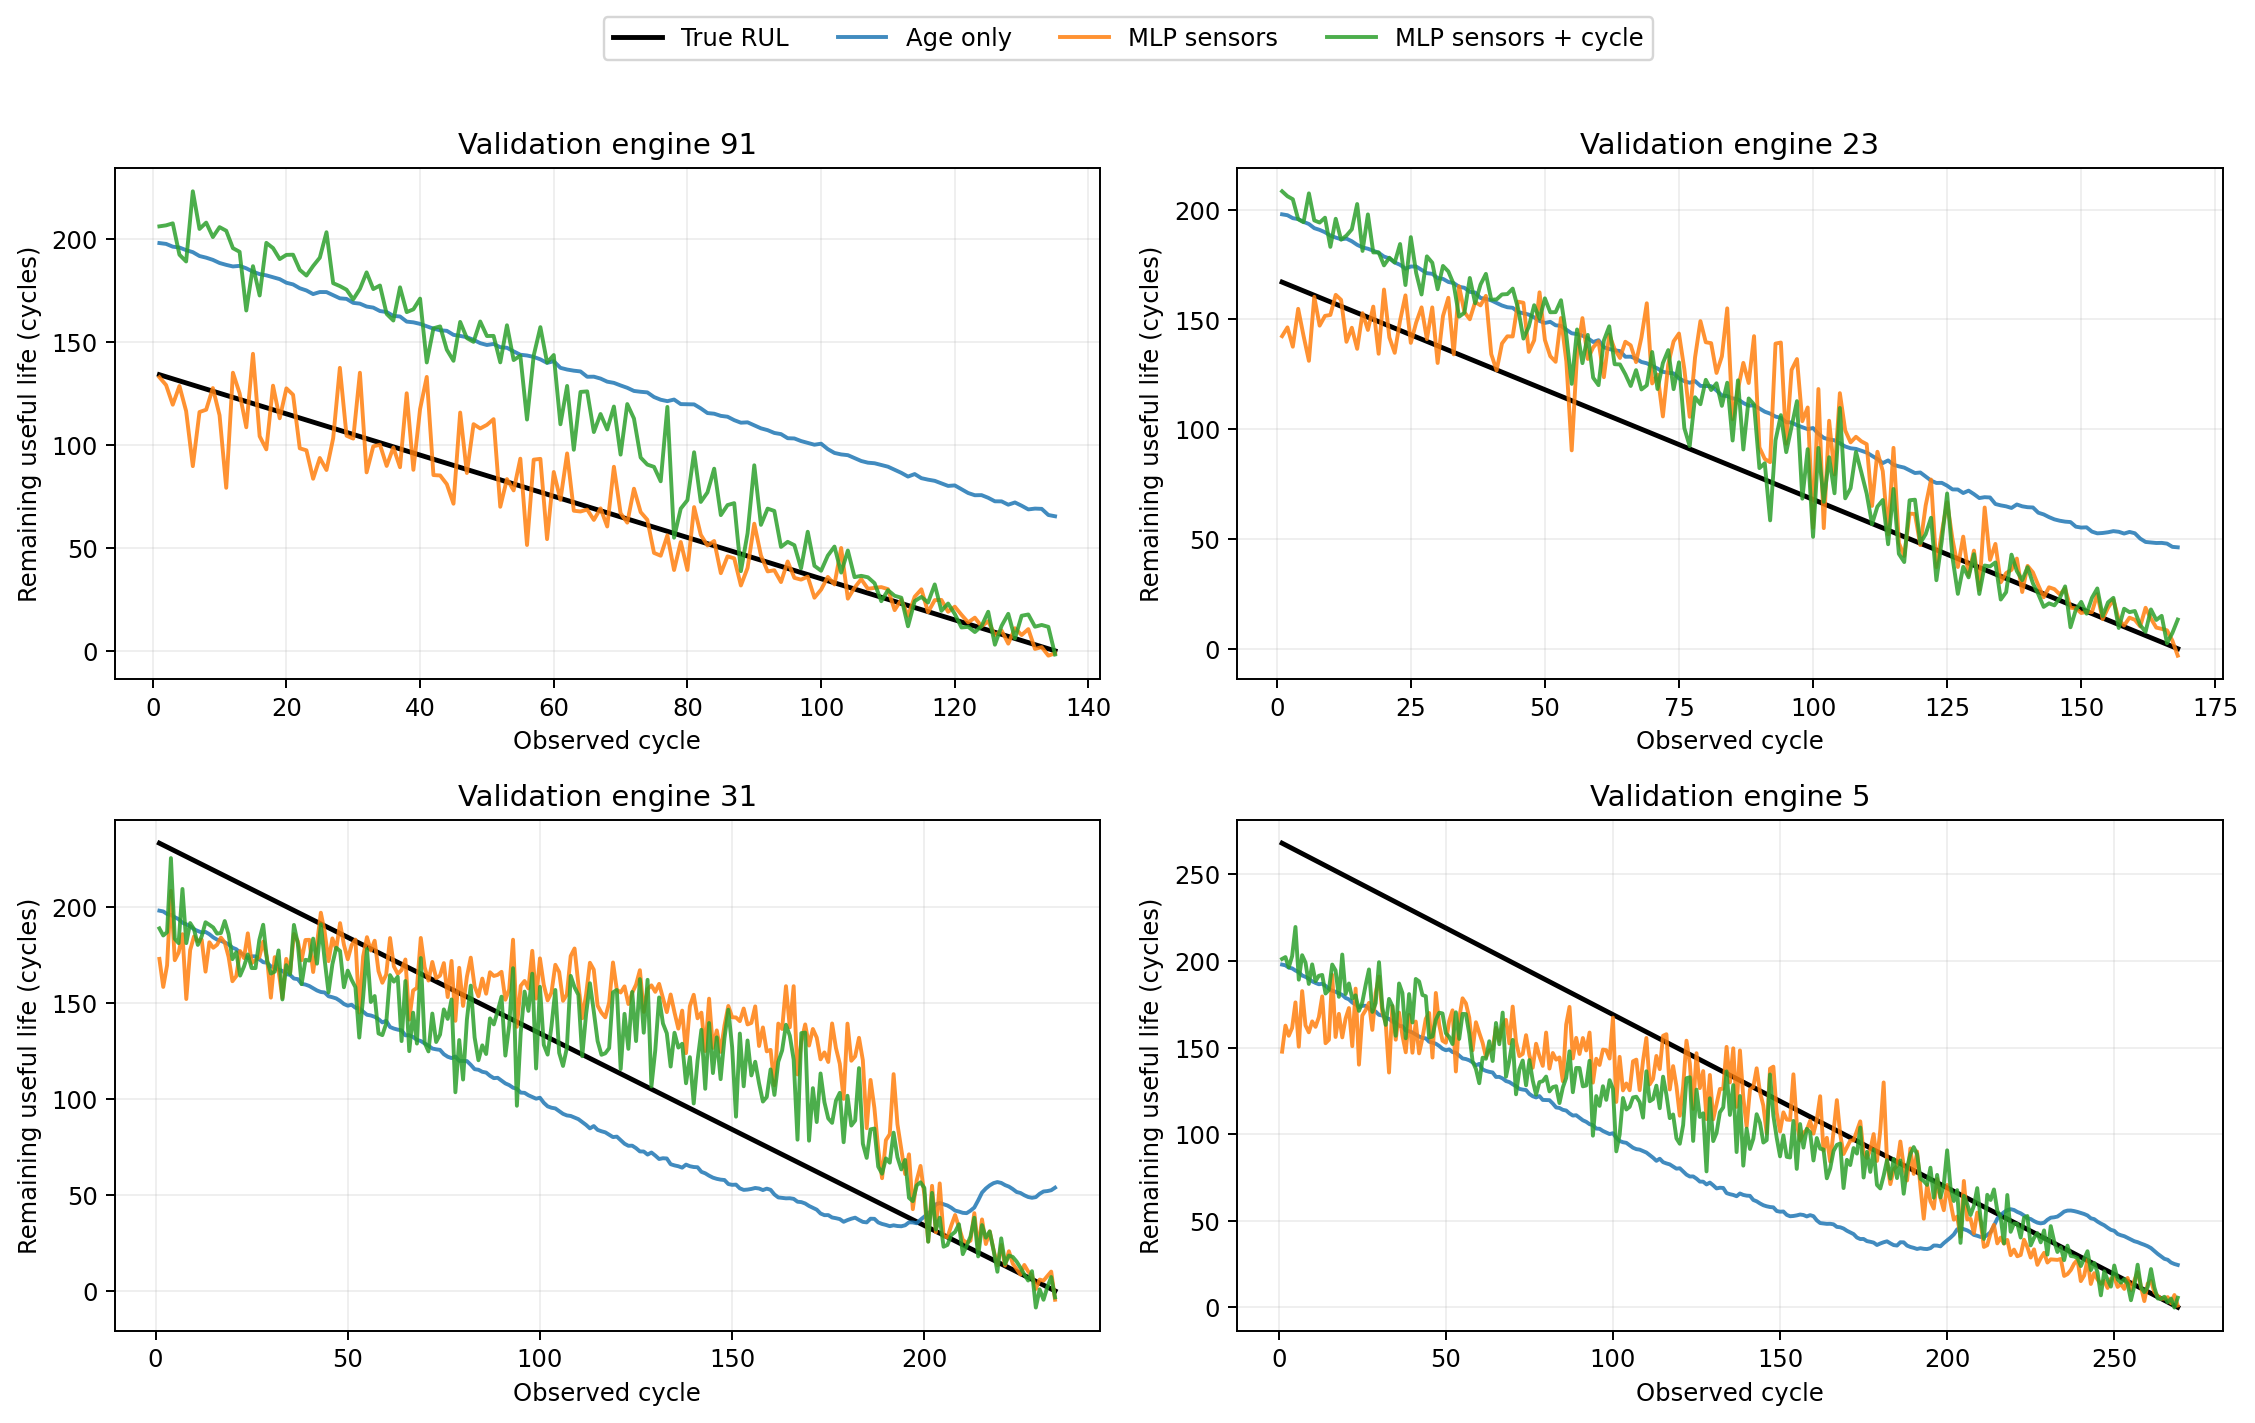
\includegraphics[width=.94\textwidth]{rul_trajectories.png}\caption{Истинный и предсказанный RUL на четырёх полностью отложенных валидационных двигателях. Для официального теста промежуточные эталонные RUL не доступны}\end{figure}
\section{Нейросетевая модель и процесс обучения}
\subsection{Архитектура и функция потерь}
MLP представляет собой полносвязную регрессионную сеть с двумя скрытыми слоями и функцией активации ReLU; выходной слой линейный. В базовом сравнении использована архитектура (48, 24), регуляризация $\alpha=1$ и алгоритм Adam с начальной скоростью обучения $10^{-3}$. Оптимизируется среднеквадратичная ошибка с L2-штрафом на веса. Отрицательные прогнозы возможны: неотрицательность RUL отдельным ограничением не обеспечивалась.

После обработки пропусков и стандартизации на обучении выполняются эпохи оптимизации. В дополнительном эксперименте явные вызовы \texttt{partial\_fit} позволяют оценивать MAE по окончании каждой эпохи на обучающих и полностью отложенных валидационных двигателях. Веса лучшей эпохи сохраняются по минимальной валидационной MAE; критерий остановки — отсутствие улучшения более 0,01 цикла в течение 22 эпох, не ранее 35-й эпохи, либо предел 160 эпох. Здесь валидация отличается от внутреннего случайного \texttt{early\_stopping} первоначального скрипта.
\subsection{Кривые обучения и насыщение точности}
\begin{figure}[H]\centering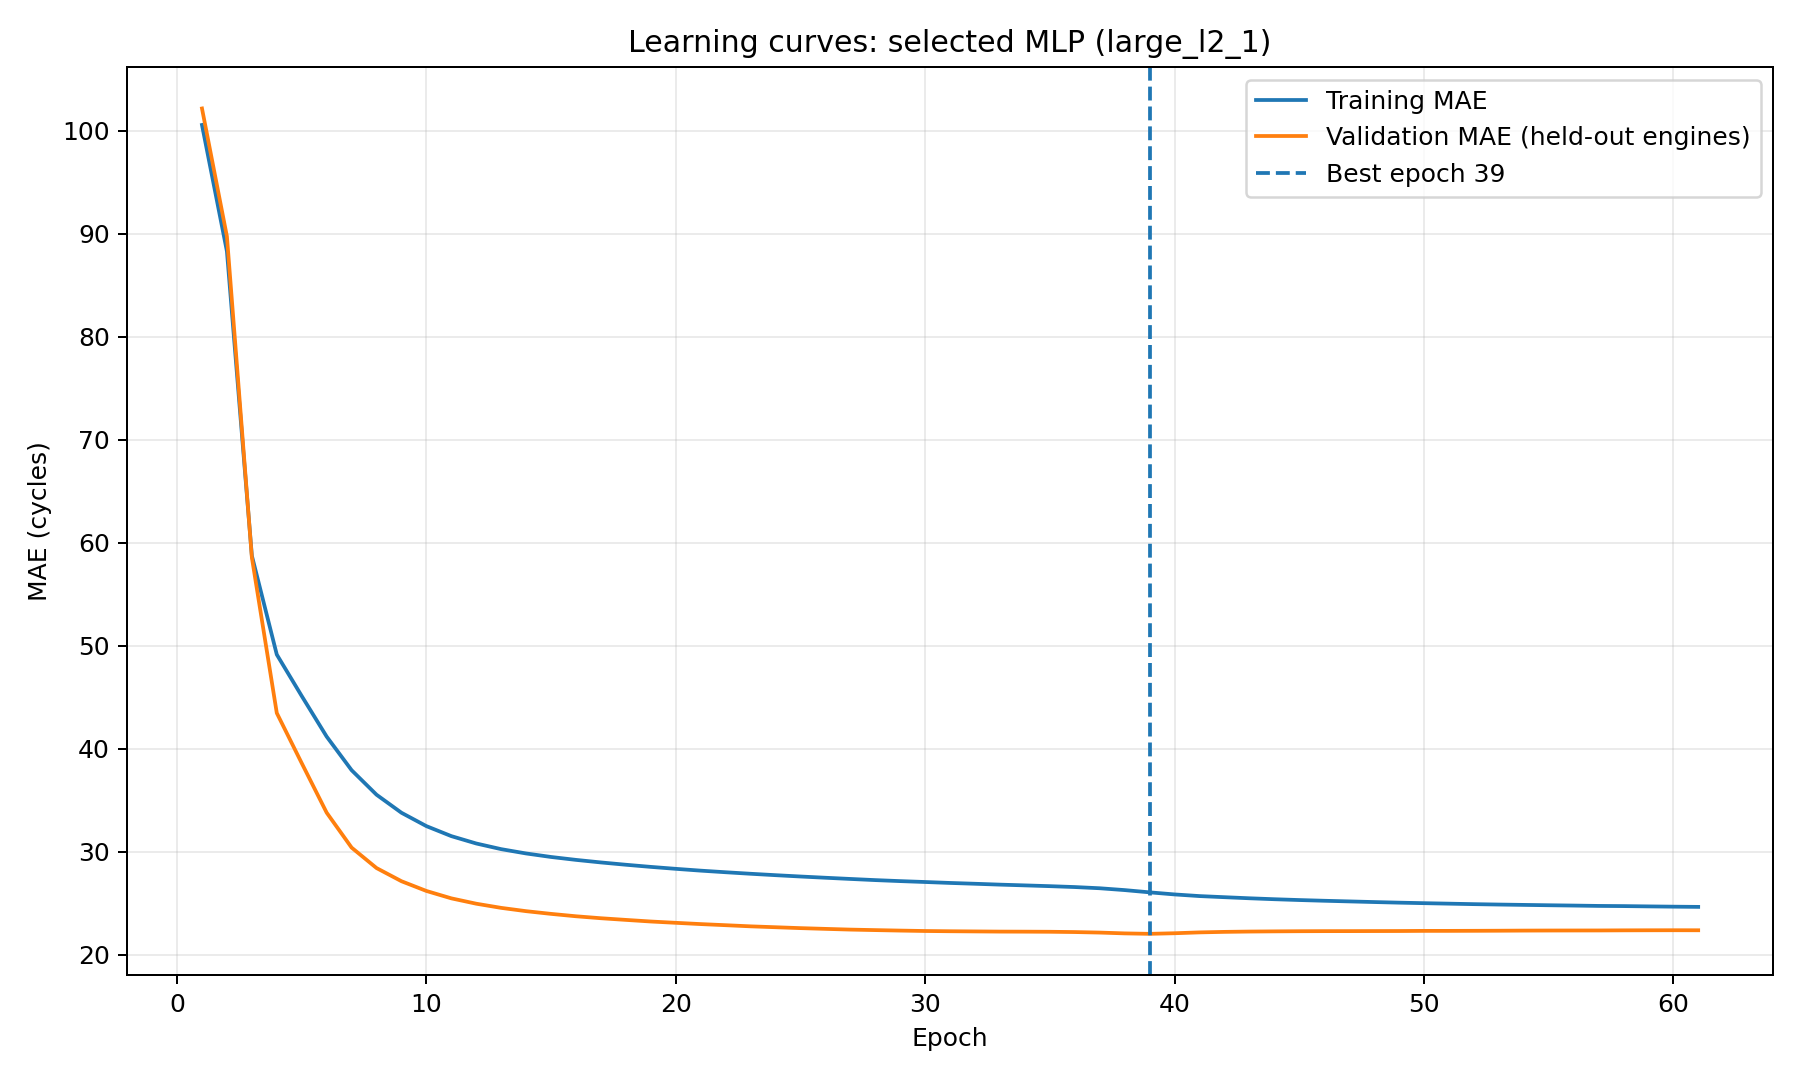
\includegraphics[width=.91\textwidth]{learning_curves.png}\caption{Кривые MAE на обучении и валидации выбранной конфигурации MLP (64, 32) с контролем по эпохам}\end{figure}
Кривые позволяют отличить уменьшение ошибки на обучении от улучшения обобщения. После некоторого числа эпох тренд валидационной MAE выходит на плато или ухудшается, хотя обучающая ошибка может продолжать уменьшаться. Поэтому выбор эпохи по обучающей ошибке недостаточен; использован отбор лучшей эпохи по независимым двигателям.
\section{Первоначальный подбор гиперпараметров}
Исследованы четыре заранее заданные конфигурации при одном и том же исходном разбиении (\texttt{seed=42}). Варьировались размеры двух скрытых слоёв и коэффициент L2-регуляризации. Это \emph{ограниченный перебор}, а не исчерпывающий поиск по всем скоростям обучения, архитектурам и количеству эпох.
\begin{table}[H]\centering\caption{Результаты подбора MLP по валидационной MAE}\begin{tabular}{lrrrr}\toprule Скрытые слои & $\alpha$ & Эпох выполнено & Лучшая эпоха & MAE\\\midrule (32, 16) & 0,1 & 95 & 73 & 22,145\\ (48, 24) & 0,1 & 86 & 64 & 22,254\\ (48, 24) & 1,0 & 66 & 44 & 22,327\\ (64, 32) & 1,0 & 61 & 39 & \textbf{22,015}\\\bottomrule\end{tabular}\end{table}
\begin{figure}[H]\centering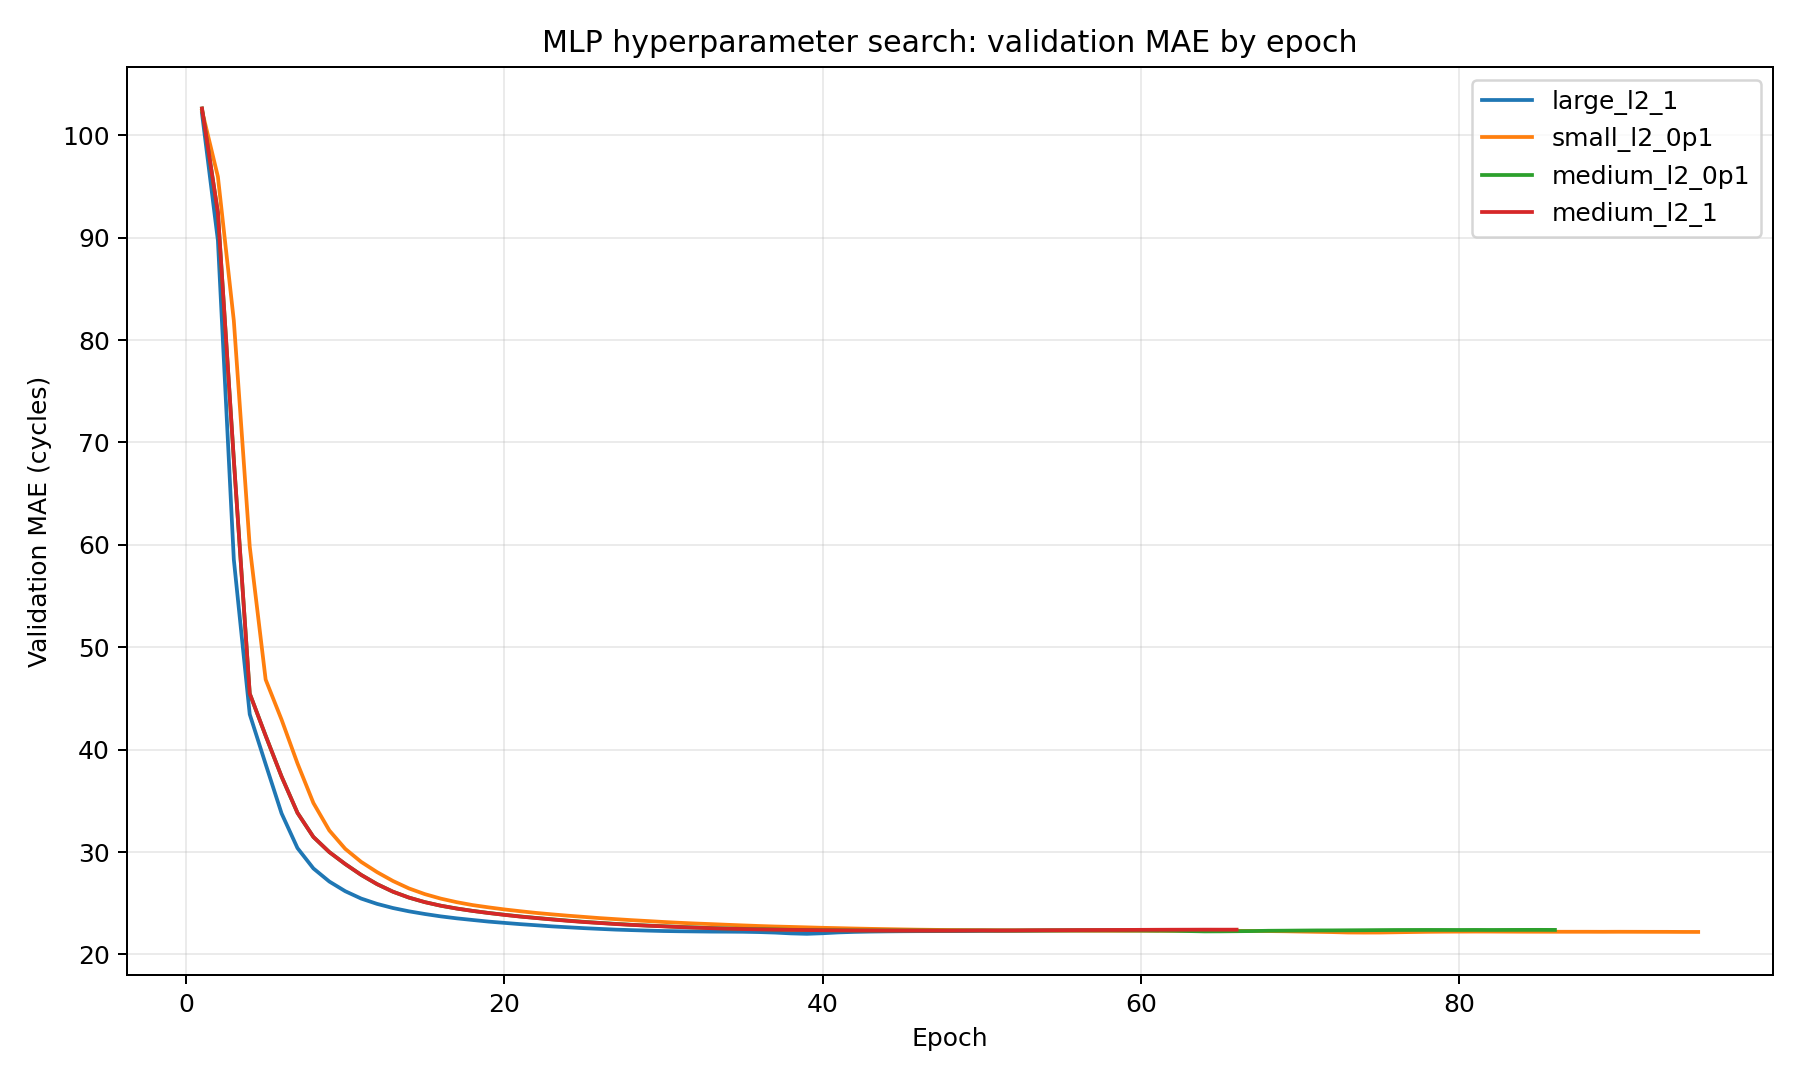
\includegraphics[width=.91\textwidth]{tuning_comparison.png}\caption{Сопоставление исследованных конфигураций MLP по валидационной MAE}\end{figure}
Конфигурация (64, 32), $\alpha=1$ дала наименьшую валидационную MAE = 22,015. После выбора она получила на официальном тесте MAE = 19,629 и RMSE = 25,699. Этот результат немного хуже первоначальной комбинированной MLP (19,458), поэтому утверждать, будто подбор улучшил тестовую точность, нельзя. Ценность эксперимента состоит в воспроизводимом протоколе отбора и анализе сходимости.
\section{Повторные разбиения по двигателям}
\subsection{Схема проверки устойчивости}
По замечанию преподавателя проведён дополнительный эксперимент на трёх значениях случайного зерна: 17, 42 и 73. Для каждого заново выбираются независимые группы двигателей и полные траектории с суммарным обучающим бюджетом не более 8\,000 циклов. Число обучающих траекторий составляет 39--40, валидационных двигателей всегда 20. Исследованы три конфигурации MLP: (32,16) при $\alpha=0{,}1$, (48,24) при $\alpha=1$ и (64,32) при $\alpha=1$. Для сопоставимости используется \texttt{max\_iter=120}, внутреннее раннее прекращение обучения и неизменная скорость $10^{-3}$.

Эти расчёты проводятся \emph{на валидационных траекториях}, а не на официальном тесте. Поскольку меняется не только начальная инициализация, но и состав обучающих и валидационных двигателей, полученная дисперсия характеризует совместную чувствительность к данным и случайности обучения, а не чистое влияние начальных весов.
\begin{table}[H]\centering\caption{MAE по отдельным разбиениям для неограниченной целевой переменной}\begin{tabular}{lrrr}\toprule Модель & seed 17 & seed 42 & seed 73\\\midrule MLP (32,16), $\alpha=0{,}1$ & 22,09 & 22,36 & 29,15\\ MLP (48,24), $\alpha=1$ & 24,40 & 22,43 & 30,48\\ MLP (64,32), $\alpha=1$ & 24,95 & 22,67 & 29,84\\\bottomrule\end{tabular}\end{table}
Для наглядности в таблице показано, что смена выборки меняет качество на несколько циклов. Одна конкретная настройка не гарантирует преимущество во всех разбиениях. Результаты не заменяют полноценные интервалы неопределённости на независимых задачах: всего три разбиения и одна процедура обучения на каждую пару «разбиение--конфигурация».
\section{Ограничение RUL сверху: эксперимент и компромисс}
\begin{table}[H]\centering\caption{Средняя MAE на валидации по трём seeds: без ограничения и cap=125}\begin{tabular}{lrrr}\toprule MLP & Без cap & Cap 125 & При малом RUL: без / cap\\\midrule (32,16), $\alpha=0{,}1$ & 24,53 & 32,98 & 6,98 / 6,55\\ (48,24), $\alpha=1$ & 25,77 & 33,25 & 8,20 / 7,31\\ (64,32), $\alpha=1$ & 25,82 & 33,03 & 8,16 / 6,17\\\bottomrule\end{tabular}\end{table}
\begin{figure}[H]\centering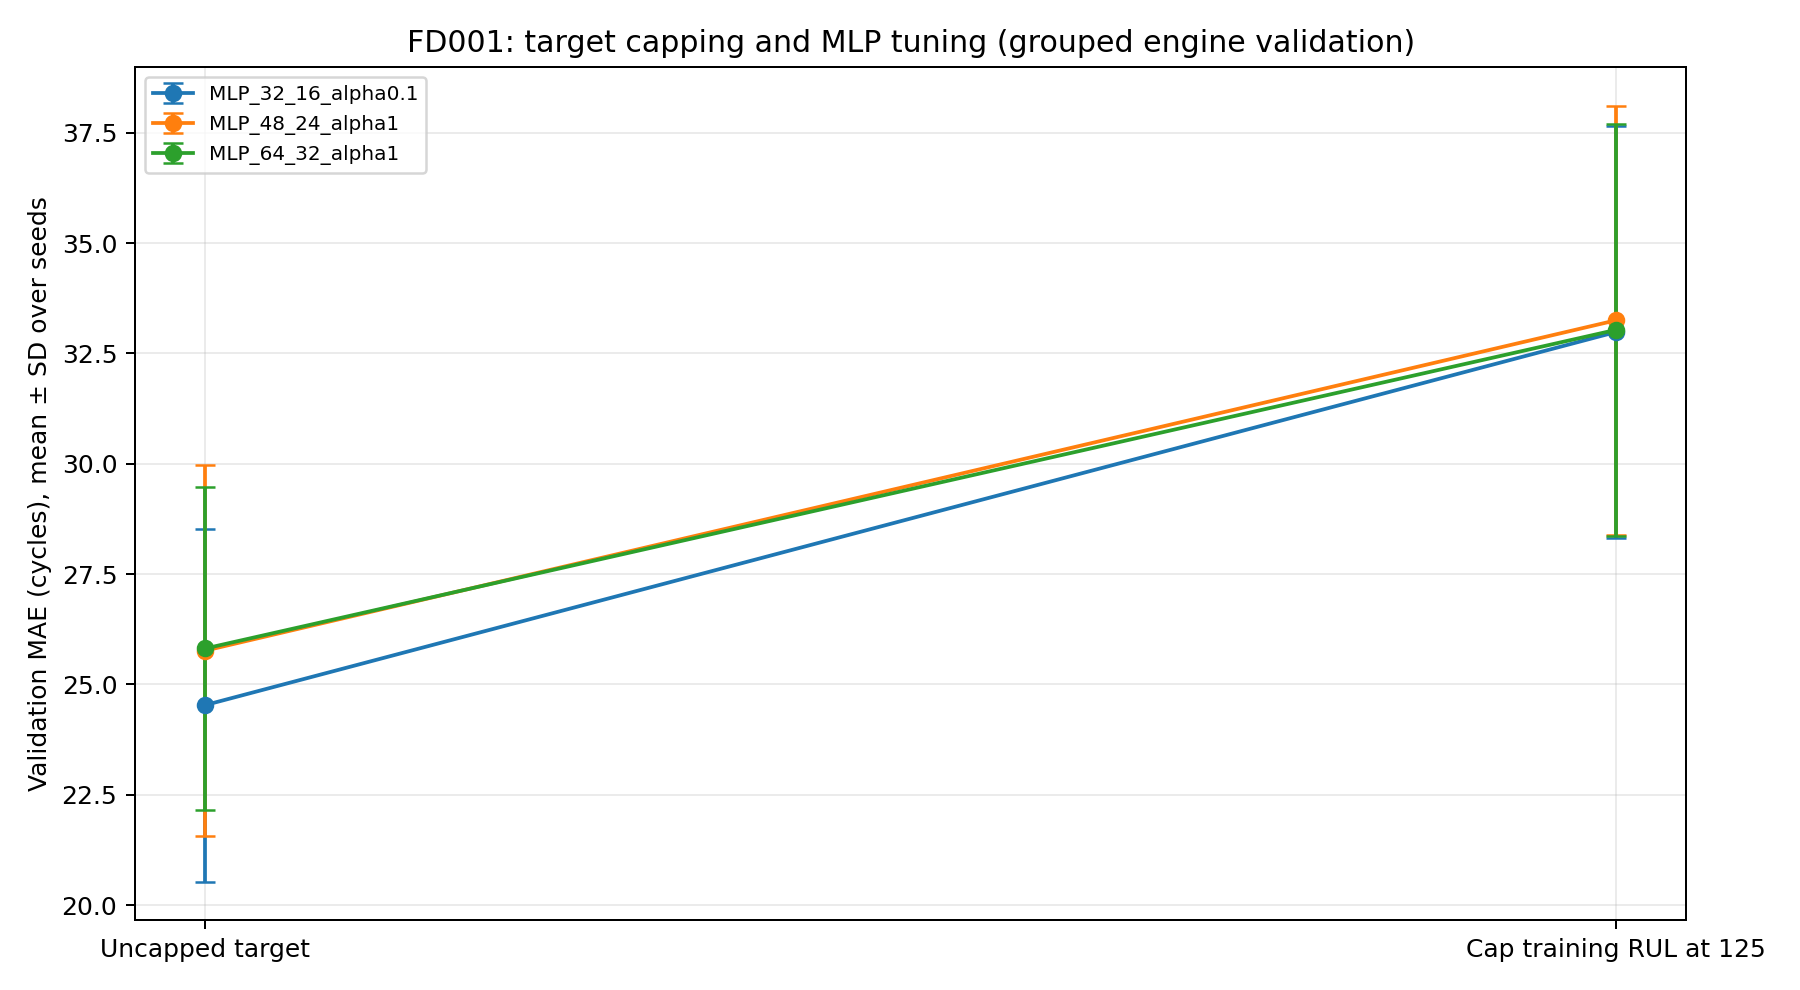
\includegraphics[width=.95\textwidth]{robustness_comparison.png}\caption{Средняя по трём seeds валидационная MAE с разбросом для разных конфигураций MLP и cap целевой переменной}\end{figure}
Из таблицы следует, что ограничение обучающей цели до 125 циклов при сравнении с \emph{неограниченным} RUL ухудшает общую MAE примерно на 7--8,5 цикла. В то же время в диапазоне RUL 0--30 средняя MAE становится несколько ниже. Следовательно, верхнее ограничение полезно рассматривать как выбор приоритета близкого отказа, а не как безусловное улучшение модели. Для честного сравнения с другими работами обязательно указывать, была ли целевая переменная ограничена и в какой шкале подсчитывается ошибка.
\section{Процентные метрики и интерпретация}
\begin{table}[H]\centering\caption{Процентные ошибки на официальном тесте, исходные четыре модели}\begin{tabular}{lrr}\toprule Модель & MAPE, \% & sMAPE, \%\\\midrule Только цикл & 80,67 & 47,85\\ Ridge, датчики & 53,07 & 38,26\\ MLP, датчики & 36,44 & \textbf{28,36}\\ MLP, датчики и цикл & \textbf{31,07} & 29,59\\\bottomrule\end{tabular}\end{table}
На официальном тесте нулевых истинных RUL среди 100 последних наблюдений нет, поэтому MAPE вычисляется по всем 100 двигателям. Минимальную MAPE имеет комбинированная MLP (31,07\%), но по sMAPE немного лучше сенсорная MLP без цикла (28,36\% против 29,59\%). Следовательно, вывод о лучшем методе зависит и от метрики. MAPE особенно чувствительна к малым истинным RUL; её нельзя интерпретировать как универсальную меру качества без указания диапазона и способа обработки нуля.

В повторных валидационных экспериментах для сравнений включены MAPE по $RUL\geq10$ и sMAPE; значения также сохраняются в таблицах \texttt{robustness\_results.csv} и \texttt{robustness\_summary.csv}. Это позволяет избежать скрытой подмены MAPE произвольным делением на $\max(y,1)$.

\section{Расширенные эксперименты по замечаниям преподавателя}
\subsection{Полная сетка настройки MLP на трёх разбиениях}
После первоначального исследования четырёх конфигураций проведён отдельный эксперимент с восьмью сочетаниями: архитектура $(32,16)$ или $(64,32)$, коэффициент регуляризации $\alpha=0{,}1$ или $1{,}0$ и скорость обучения $\eta=0{,}0005$ или $0{,}001$. Каждый вариант проверялся на \emph{трёх} разбиениях (17, 42, 73): всего 24 обучения. Для одинакового вычислительного бюджета установлен предел 100 эпох и внутреннее раннее прекращение при отсутствии улучшения в течение 12 итераций. Предел эпох не означает, что все сети полностью сошлись: такие запуски интерпретируются как сравнение при заданном бюджете, а не доказательство глобального оптимума.

\begin{table}[H]\centering\caption{Расширенная сетка MLP: средняя MAE и СКО по трём разбиениям}
\begin{tabular}{lrrr}\toprule Архитектура & $\alpha$ & $\eta$ & MAE, циклы\\\midrule
(32,16) & 0,1 & 0,0005 & $25{,}54\pm4{,}73$\\
(32,16) & 0,1 & 0,0010 & $\mathbf{24{,}53\pm4{,}00}$\\
(32,16) & 1,0 & 0,0005 & $25{,}54\pm4{,}73$\\
(32,16) & 1,0 & 0,0010 & $24{,}72\pm3{,}88$\\
(64,32) & 0,1 & 0,0005 & $25{,}60\pm3{,}95$\\
(64,32) & 0,1 & 0,0010 & $25{,}83\pm3{,}73$\\
(64,32) & 1,0 & 0,0005 & $25{,}60\pm4{,}01$\\
(64,32) & 1,0 & 0,0010 & $25{,}76\pm3{,}68$\\\bottomrule\end{tabular}
\end{table}
\begin{figure}[H]\centering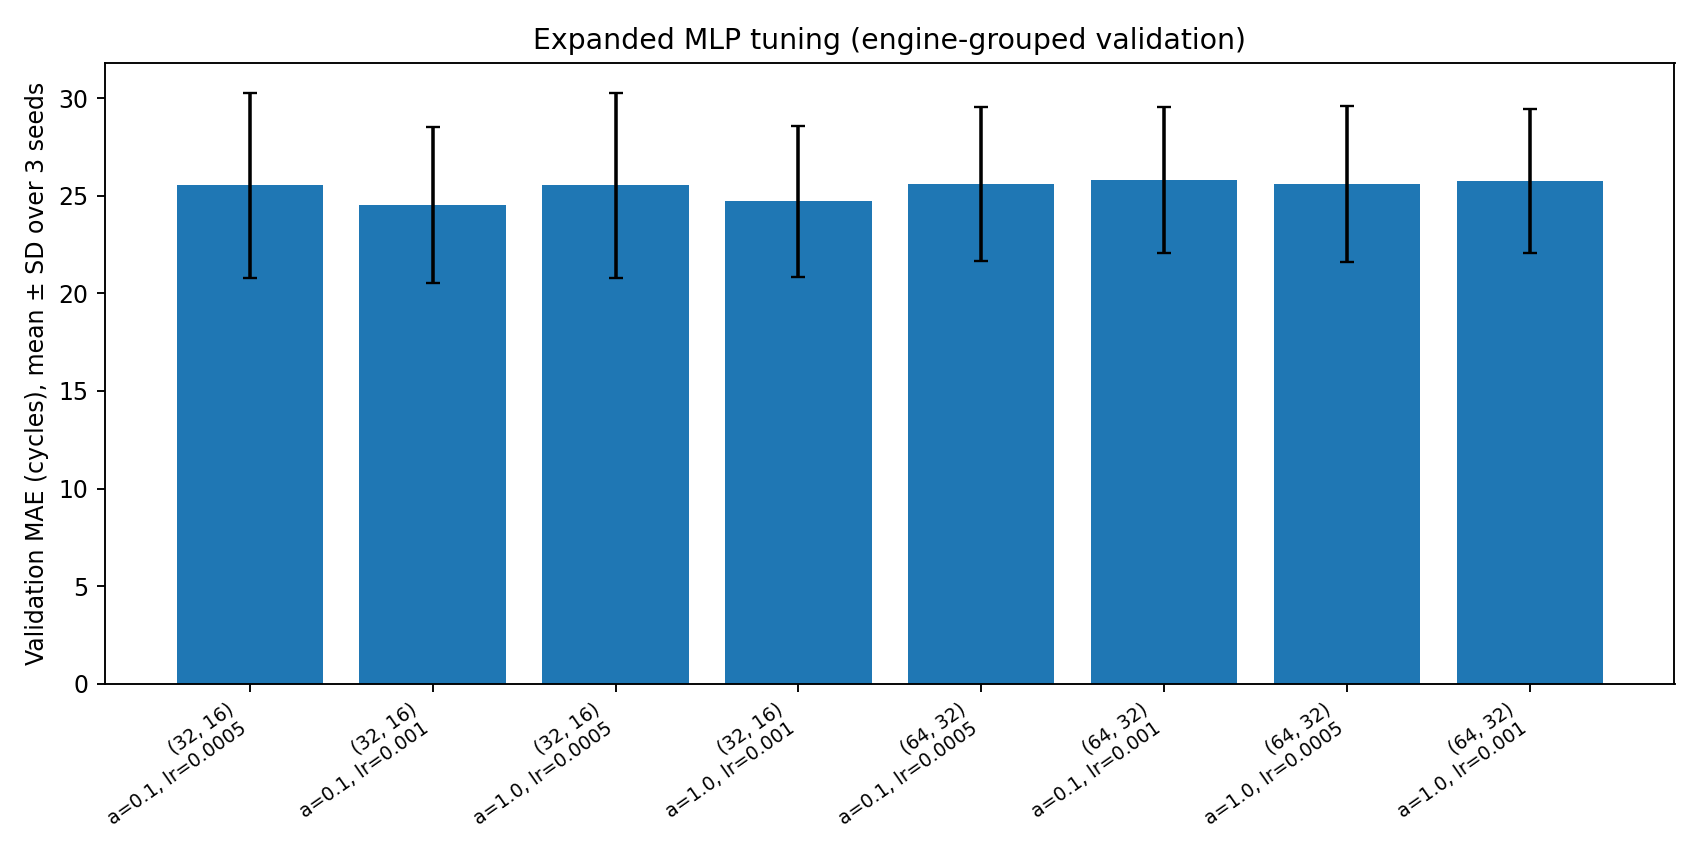
\includegraphics[width=.94\textwidth]{extended_tuning.png}\caption{Влияние архитектуры, регуляризации и скорости обучения на MAE; разброс между тремя разбиениями}\end{figure}
Наименьшую \emph{среднюю валидационную} MAE (24,53) получила сеть $(32,16)$, $\alpha=0{,}1$, $\eta=0{,}001$. Преимущество перед близкой конфигурацией $(32,16)$, $\alpha=1$, $\eta=0{,}001$ составляет всего 0,19 цикла, существенно меньше разброса между разбиениями ($\approx4$ цикла). Поэтому нельзя считать тонкую разницу настроек статистически доказанной. Существеннее меняется состав отложенных двигателей.

\begin{figure}[H]\centering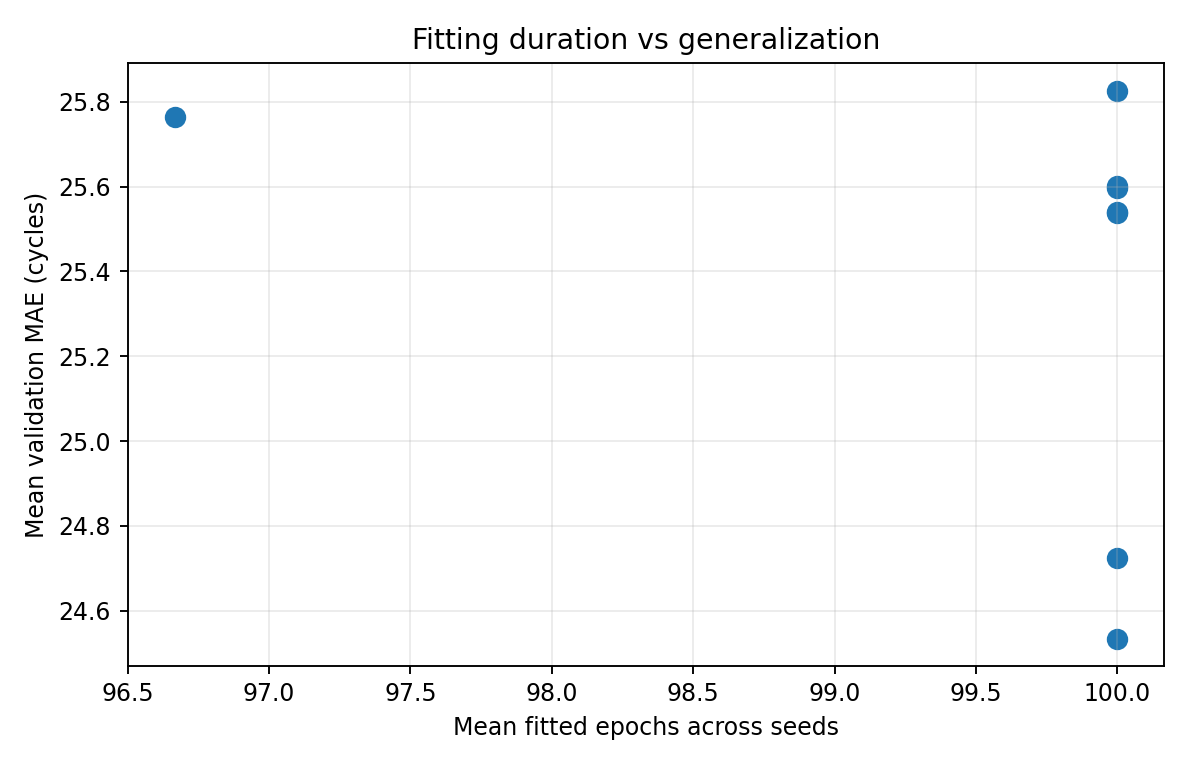
\includegraphics[width=.77\textwidth]{extended_plateau.png}\caption{Связь числа фактически выполненных эпох и средней валидационной MAE; сравнение ограничено 100 эпохами}\end{figure}
Диагностика плато: повышение сложности с $(32,16)$ до $(64,32)$ и изменение регуляризации не обеспечили устойчивого уменьшения MAE. На кривых обучения исходного эксперимента также видны эпохи, после которых ошибка обучения убывает, но валидация уже не улучшается. Наиболее осторожная интерпретация — \emph{плато обобщения в исследованном диапазоне}, а не принципиальный предел точности любых MLP.

\subsection{Пять вариантов верхнего ограничения обучающего RUL}
Выбранная по средней валидации конфигурация MLP $(32,16)$, $\alpha=0{,}1$, $\eta=0{,}001$ дополнительно обучена для $c\in\{100,125,150,200\}$ и без ограничения, с теми же тремя разбиениями. Это ещё 15 обучений. Для оценки \emph{всегда} используется настоящий, неограниченный RUL валидационных двигателей, а сами предсказания не обрезаются сверху. Таким образом, изменяется \emph{только обучающая цель}, а не способ подсчёта качества.
\begin{table}[H]\centering\caption{Ограничение обучающего RUL: MAE по трём разбиениям}
\begin{tabular}{lrr}\toprule Верхняя граница & Общая MAE, циклы & MAE при RUL $\leq30$\\\midrule
Без ограничения & $\mathbf{24{,}53\pm4{,}00}$ & $6{,}98\pm0{,}23$\\
100 & $41{,}19\pm4{,}61$ & $6{,}47\pm0{,}94$\\
125 & $32{,}98\pm4{,}68$ & $6{,}55\pm0{,}70$\\
150 & $28{,}18\pm4{,}53$ & $\mathbf{6{,}34\pm0{,}02}$\\
200 & $25{,}01\pm3{,}94$ & $6{,}60\pm0{,}08$\\\bottomrule\end{tabular}
\end{table}
\begin{figure}[H]\centering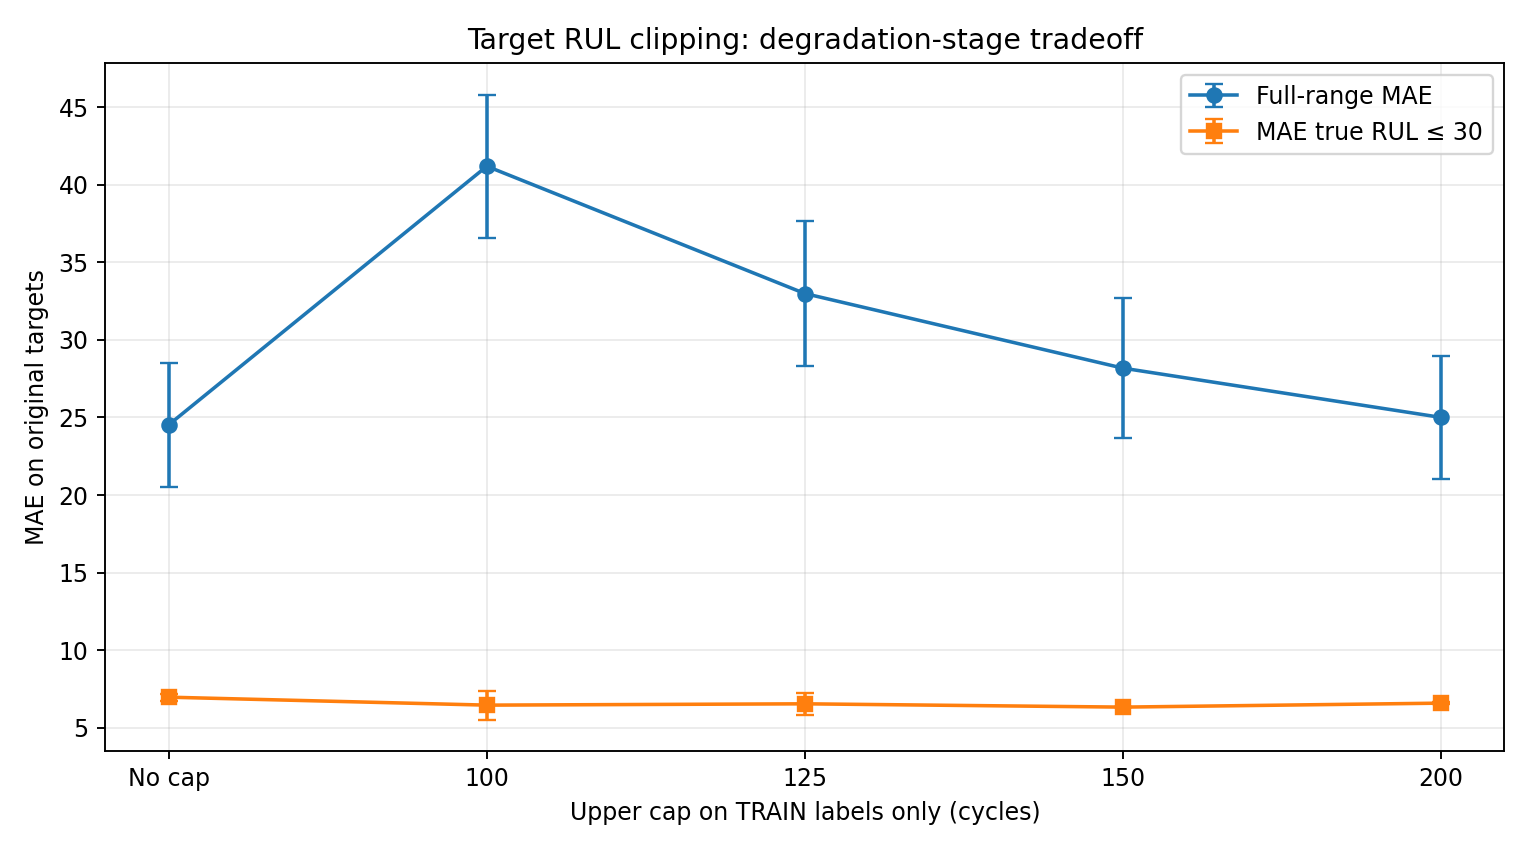
\includegraphics[width=.94\textwidth]{extended_rul_caps.png}\caption{Компромисс между точностью по всей шкале RUL и близостью отказа при разных ограничениях обучающей цели}\end{figure}
Из таблицы видно, что чрезмерное ограничение до 100 резко увеличивает общую MAE ($41{,}19$ против $24{,}53$ циклов), хотя в малом RUL ошибка ниже. При $c=150$ минимальная MAE в диапазоне $0$--$30$, однако общая MAE хуже, чем без ограничения. Приведённые СКО отражают разброс между тремя одновременно изменяющимися разбиениями и инициализациями, а не доверительные интервалы по независимым экспериментальным установкам.

\subsection{Официальный тест и процентные ошибки расширенной модели}
После выбора гиперпараметров \emph{только по валидации} конфигурация без ограничения обучена при разбиении seed 42 и оценена на стандартных 100 тестовых двигателях. Получены MAE $=18{,}989$, RMSE $=25{,}237$ циклов, MAPE $=33{,}981\%$ и sMAPE $=32{,}321\%$. По сравнению с исходной MLP (MAE $=19{,}458$, MAPE $=31{,}07\%$) абсолютная ошибка стала несколько ниже, но процентная — выше. Это подчёркивает зависимость понятия лучшей модели от метрики; тестовые ответы \emph{не использовались} для выбора параметров.

\subsection{Вычислительный бюджет и воспроизводимость}
Для расширенной сетки выполнены 24 обучения, для эксперимента с верхней границей -- 15, всего 39 запусков. Лимит в 8\,000 обучающих циклов соблюдён в каждом разбиении: 7\,933 при seed 17, 7\,954 при seed 42, 7\,879 при seed 73. В каждом случае отложены 20 полных двигателей, а параметры стандартизации изучаются исключительно по обучающим. Таблицы \texttt{extended\_grid.csv}, \texttt{extended\_grid\_summary.csv}, \texttt{extended\_caps.csv} и \texttt{extended\_caps\_summary.csv} вместе со скриптом \texttt{extended\_study.py} позволяют независимо проверить весь расширенный эксперимент.

\section{Ограничения и обсуждение}
Работа основана на симуляторе FD001: один режим и один тип повреждения не позволяют без дополнительной проверки переносить числа MAE на реальные авиационные двигатели. Входы моделей учитывают текущие датчики и цикл, но не используют временные окна, накопленные производные или рекуррентную архитектуру. Базовая возрастная модель — случайный лес по номеру цикла, то есть утверждение о превосходстве датчиков относится к выбранному набору сравниваемых алгоритмов.

Внутреннее \texttt{early\_stopping} библиотеки sklearn в некоторых запусках отбирает случайные строки из обучающих траекторий и не обеспечивает независимости по двигателям. Основная внешняя валидация, однако, строго отделена по идентификаторам двигателей. В дополнительном исследовании разбиения по seeds меняются вместе с инициализациями, поэтому нельзя изолировать вклад каждого фактора случайности. Расширенная сетка гиперпараметров охватывает два варианта размеров скрытых слоёв, два значения регуляризации и две скорости обучения; рассматриваются все четыре значения ограничения RUL и отсутствие ограничения. Более широкие архитектуры, другие оптимизаторы и независимые многократные инициализации при неизменном составе двигателей остаются предметом дальнейшего исследования. В одном исходном MLP обучение ограничилось пределом итераций, не достигнув критерия сходимости.

Важно не считать повторные валидации независимыми финальными тестами: выбор модели по ним допустим, но итоговый официальный тест должен использоваться только для отчётной оценки. Различия в исследовании cap отражают одновременно изменение постановки обучающей цели и выбранную функцию потерь. Дополнительные повторные разбиения и интервалы позволили бы уточнить статистическую устойчивость выигрыша.
\section*{ЗАКЛЮЧЕНИЕ}\addcontentsline{toc}{section}{Заключение}
\begin{enumerate}[leftmargin=1.3cm]
\item В первоначальном контролируемом сравнении MLP с датчиками и циклом достигает MAE=19,46 на штатном тесте FD001, уменьшая ошибку относительно модели только по циклу на 33,3\%.
\item При истинном RUL 0--30 сенсорные нейросети значительно точнее возрастной модели: MAE 9,24--9,35 против 32,57 цикла. Этот выигрыш нельзя автоматически переносить на большие значения RUL.
\item Кривые обучения подтверждают необходимость контролировать качество на отложенных двигателях. Лучшая из четырёх проверенных настроек — MLP (64,32), $\alpha=1$, эпоха 39, валидационная MAE=22,015; её тестовая MAE=19,629, что не лучше исходной 19,458.
\item По трём seeds качество заметно меняется. Ограничение обучающего RUL до 125 уменьшает ошибку при близком отказе для исследованных конфигураций, но ухудшает общую ошибку по полному истинному RUL.
\item Расширенная сетка из восьми настроек на трёх разбиениях и эксперимент с пятью уровнями cap (всего 39 запусков) показывают, что лучшие настройки и компромисс при малом RUL зависят от критерия: cap 150 улучшил MAE при RUL до 30, но ухудшил общую MAE.\item Добавлены процентные метрики: на официальном тесте MAPE исходной комбинированной MLP=31,07\%. Для полных траекторий при нулевом RUL MAPE следует считать только по ненулевым значениям или использовать sMAPE и порог $RUL\geq10$.
\end{enumerate}
Таким образом, данные датчиков действительно несут дополнительную информацию об износе двигателя в рамках FD001. Научно корректная оценка требует одновременно проверять среднюю ошибку, качество при малом RUL, чувствительность к разбиению и последствия изменения определения обучающей цели.
\section*{СПИСОК ИСПОЛЬЗОВАННЫХ ИСТОЧНИКОВ}\addcontentsline{toc}{section}{Список использованных источников}
\begin{enumerate}[leftmargin=1.3cm]
\item Saxena A., Goebel K., Simon D., Eklund N. Damage propagation modeling for aircraft engine run-to-failure simulation // International Conference on Prognostics and Health Management. 2008.
\item NASA Prognostics Center of Excellence. Turbofan Engine Degradation Simulation Data Set (C-MAPSS). NASA Prognostics Data Repository.
\item Pedregosa F. et al. Scikit-learn: Machine Learning in Python // Journal of Machine Learning Research. 2011. Vol. 12. P. 2825--2830.
\item Kingma D. P., Ba J. Adam: A Method for Stochastic Optimization // ICLR. 2015.
\item Bishop C. M. Pattern Recognition and Machine Learning. Springer, 2006.
\end{enumerate}
\section*{ПРИЛОЖЕНИЕ А. Воспроизводимость}\addcontentsline{toc}{section}{Приложение А. Воспроизводимость}
Исходный архив \texttt{CMAPSSData.zip} поставляется отдельно; в публикацию результатов не включён. Команды запуска из корневого каталога проекта:
\begin{verbatim}
python -m pip install -r requirements.txt
python experiment.py --zip CMAPSSData.zip --out .
python train_mlp_tuning.py --zip CMAPSSData.zip --out .
python robustness_study.py --zip CMAPSSData.zip --out .
python extended_study.py --zip CMAPSSData.zip --out .
\end{verbatim}
Запуски строят таблицы ошибок, матрицы предсказаний, графики обучения, результаты подбора гиперпараметров и проверки по трём seeds. Приведённые в PDF цифры взяты из сохранённых CSV-артефактов репозитория. Для воспроизведения на другой версии библиотек возможны небольшие отличия из-за оптимизации MLP и аппаратно-зависимых вычислений.
\end{document}
